%% LyX 2.3.1-1 created this file.  For more info, see http://www.lyx.org/.
%% Do not edit unless you really know what you are doing.
\documentclass[english,hebrew]{article}
\usepackage[T1]{fontenc}
\usepackage[utf8]{inputenc}
\usepackage{babel}
\usepackage{amstext}
\usepackage{amssymb}
\usepackage{graphicx}
\usepackage[unicode=true]
 {hyperref}

\makeatletter

%%%%%%%%%%%%%%%%%%%%%%%%%%%%%% LyX specific LaTeX commands.
%% Because html converters don't know tabularnewline
\providecommand{\tabularnewline}{\\}

\makeatother

\begin{document}
\title{ריבוע הקסם של פרס-מרמין - איך זה עובד?}
\maketitle
\begin{description}
\item [{קטגוריות:}] פיזיקה, תורת הסיבוכיות
\item [{תגים:}] חישוב קוונטי
\item [{מזהה:}] \L{mermin\_peres\_magic\_square\_solution}
\end{description}

\section{חלק ראשון, ובו אנחנו נזכרים בריבוע הקסם של פרס ומרמין}

\L{\href{https://gadial.net/2020/01/31/mermin_peres_magic_square/}{לא מזמן}}
כתבתי פוסט שמציג את \textquotedblright ריבוע הקסם\textquotedblleft{}
של פרס-מרמין. ריבוע הקסם הזה הוא המחשה לאתגר כלשהו שחישוב קוונטי מאפשר
לנו לפתור בזמן שחישוב \textquotedblright קלאסי\textquotedblleft{} לא
מסוגל לפתור אותו. לא נכנסתי לפרטים הטכניים של הפתרון הקוונטי כי היו
חסרים לי היסודות של חישוב קוונטי שבהם משתמשים כאן )והפוסט על ריבוע
הקסם נכתב בתור תירוץ לתת אותם(. עכשיו \L{\href{https://gadial.net/2020/02/28/what_is_a_qubit/}{כתבתי פוסטים}}
על היסודות הללו ואפשר לגשת חזרה אל ריבוע הקסם ולהסביר בדיוק איך ולמה
זה עובד.

אני אנסה לנקוט פה גישה הדרגתית - להתחיל מלהסביר את הרעיון הכללי, ולאט
לאט לפרוט אותו לפרוטות ולהסביר איך זה עובד ברמה הטכנית ביותר. גם אם
לא מחזיקים מעמד יותר רחוק מתחילת הפוסט, אני מקווה שזה כבר מספיק כדי
להבין מה הולך פה ואיך עובד הקסם.

נתחיל עם תזכורת למשחק ריבוע הקסם. זה משחק לשני שחקנים - אליס ובוב.
הם מקבלים לוח משחק שנראה כך:

\L{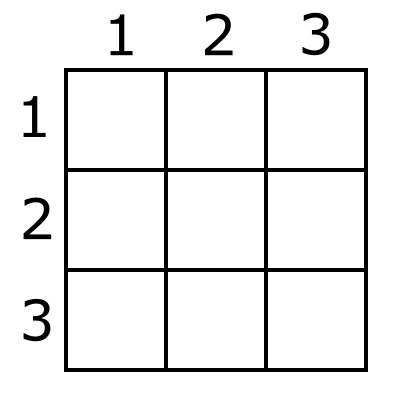
\includegraphics{C:/Users/gadia/Dropbox/Websites/blog/assets/img/2020/01/magic_square1}}

ניתנת לאליס ובוב ההזדמנות לתאם ביניהם עניינים, ואז מכניסים אותם לחדרים
נפרדים ואין להם יותר דרכי תקשורת \textquotedblright קלאסיות\textquotedblleft{}
)הם לא יכולים לדבר, אין להם חיבור אינטרנט וכו'(

אחרי שאליס נכנסת לחדר נותנים לה מספר שנבחר באקראי )בהתפלגות אחידה(
בין {\beginL 1\endL} ל-{\beginL 3\endL} והיא צריכה לצבוע את \textbf{השורה}
שזה המספר שלה, כך שבשורה יהיה \textbf{מספר זוגי} של משבצות אדומות,
כלומר משבצות עם \L{$-1$} )או {\beginL 0\endL} או {\beginL 2\endL}(.
גם בוב מקבל מספר אקראי בין {\beginL 1\endL} ל-{\beginL 3\endL} והוא
צריך לצבוע את \textbf{העמודה} שזה המספר שלה, כך שבעמודה יהיה \textbf{מספר
אי זוגי} של משבצות אדומות. והנה האתגר: לא משנה איזה שורה ועמודה אליס
ובוב קיבלו, תהיה בדיוק משבצת אחת שמשותפת לשניהם. הם צריכים לצבוע את
הצביעות שלהם כך שאותה משבצת נצבעת \textbf{באותו הצבע}. אם הם הצליחו
- הם מנצחים. אם הם נכשלו - הם מפסידים.

הנה דוגמא למשחק שהסתדר טוב מבחינת אליס ובוב:

\L{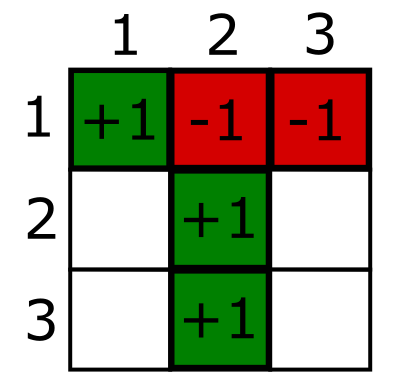
\includegraphics{C:/Users/gadia/Dropbox/Websites/blog/assets/img/2020/01/magic_square2}}

עכשיו, כל עוד אנחנו מתבססים על חישוב \textquotedblright קלאסי\textquotedblleft{}
לא משנה כמה תיאום אליס ובוב יעשו מראש, הם עדיין עלולים להפסיד במשחק
הזה. זה בגלל שאי אפשר למצוא צביעה של הלוח שבה התנאי של אליס ובוב מתקיים
תמיד. הנה נסיון אחד שנכשל:

\L{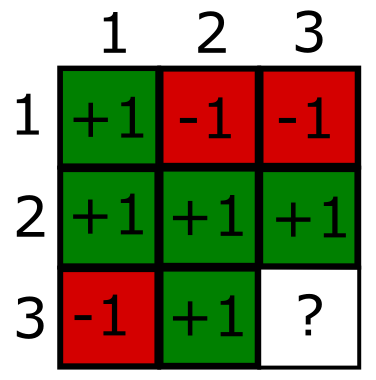
\includegraphics{C:/Users/gadia/Dropbox/Websites/blog/assets/img/2020/01/magic_square3}}

המשבצת \L{$\left(3,3\right)$} צריכה להיצבע באדום )\L{$-1$}( כדי
שהקריטריון של אליס יתקיים; היא צריכה להיצבע בירוק )\L{$+1$}( כדי
שהקריטריון של בוב יתקיים. אם אליס ובוב יוכנסו לחדרים נפרדים וההגרלה
תיתן לשניהם את שורה/עמודה {\beginL 3\endL} והם ינסו לצבוע על פי הטבלה
שלהלן, הם יפסידו כי הם ייאלצו לצבוע את המשבצת \L{$\left(3,3\right)$}
בצורה לא עקבית.

אז איך חישוב קוונטי עוזר לאליס ובוב? או, טוב ששאלתם.

\section{חלק שני, ובו אנחנו שוזרים קיוביטים}

לפני שמכניסים אותם לחדרים, אליס ובוב הולכים לחלוק ביניהם שני קיוביטים
שזורים, כלומר לשתף את המצב הקוונטי \L{$\frac{\left|00\right\rangle +\left|11\right\rangle }{\sqrt{2}}$}.
אליס תקבל את הקיוביט השמאלי ובוב יקבל את הקיוביט הימני. בצורה הזו
הם \textquotedblright מרמים את המערכת\textquotedblleft{} - אסור להם
לתקשר אינפורמציה כלשהי, אבל אם אליס מודדת את הקיוביט שלה, תוצאת המדידה
תשפיע על הקיוביט של בוב: אם אליס מודדת בבסיס \L{$Z$} ומקבלת \L{$\left|0\right\rangle $}
גם הקיוביט של בוב יקרוס למצב \L{$\left|0\right\rangle $}; אם היא
מקבלת \L{$\left|1\right\rangle $} גם הקיוביט של בוב יקרוס ל-\L{$\left|1\right\rangle $}.
בצורה הזו אליס ובוב הולכים לייצר ביניהם את התיאום שנדרש כדי שהתשובה
שיתנו למשבצת המשותפת שלהם תהיה זהה.

הפסקה שלעיל נועדה לא רק להסביר מה הולך כאן אלא לשמש בתור סוג של \textquotedblright שומר
סף\textquotedblleft{} - אם קראתם אותה ולא הבנתם מה אני רוצה מהחיים
שלכם, זה אומר שכדאי לכם לחזור קודם על הרקע הבסיסי של חישוב קוונטי
שהצגתי בפוסטים הקודמים; בהמשך הפוסט אני אניח שהמושגים שהשתמשתי בהם
שם הם מוכרים מספיק כדי שנוכל להתחיל לעבוד איתם.

הכל בסדר עכשיו? יפה, אז בואו נסבך את הסיפור \textbf{טיפה}: מה שאליס
ובוב הולכים לחלוק הוא לא זוג שזור אחד, אלא \textbf{שני} זוגות שזורים.
כלומר, לאליס יש שני קיוביטים ולבוב יש שני קיוביטים ואיכשהו הקיוביטים
של אליס יכולים להשפיע על הקיוביטים של בוב. בפרט, המערכת הקוונטית הכוללת
שעליה אנחנו מדברים כאן היא מערכת בת \textbf{ארבעה} קיוביטים; אבל רוב
הזמן אני אתייחס רק לזוג הקיוביטים של אליס או בוב ואתעלם מקיום הזוג
השני, כי זה שומר את ההצגה המתמטית פשוטה יותר.

כדי לשמור את המתמטיקה יפה, אני איעזר בסימונים סטנדרטיים: המצב הקוונטי
\L{$\frac{\left|0\right\rangle +\left|1\right\rangle }{\sqrt{2}}$},
של קיוביט בודד בסופרפוזיציה אחידה, מסומן בתור \L{$\left|+\right\rangle \triangleq\frac{\left|0\right\rangle +\left|1\right\rangle }{\sqrt{2}}$}.
אליס מתחילה את המשחק עם \textbf{שני} קיוביטים כאלו, שאין קשר בין שניהם;
הדרך שבה משלבים שני קיוביטים לא קשורים כאלו למערכת אחת היא בעזרת \textbf{מכפלה
טנזורית}, \L{$\left|+\right\rangle \otimes\left|+\right\rangle $},
וכדי לשמור את הסימון פשוט אנחנו כותבים \L{$\left|++\right\rangle $}
בשביל לתאר את המערכת הזו.

עכשיו אליס מקבלת את מספר השורה שעליה לסמן. היא פועלת בצורה שונה בהתאם
למספר השורה שקיבלה:
\begin{enumerate}
\item אליס מודדת את המצב הקוונטי שלה בבסיס \L{$Z$}.
\item אליס מודדת את המצב הקוונטי שלה בבסיס \L{$X$}.
\item אליס מודדת את המצב הקוונטי שלה בבסיס מסובך יותר, שאסביר עוד מעט מהו.
\end{enumerate}
המדידות הללו מחזירות \textbf{במובן מסויים} מצב בסיס קוונטי כלשהו.
השאלה \textquotedblright איזה מצב בסיס\textquotedblleft{} תלויה בבסיס
המדידה, כלומר מה שאפשר לקבל בשורה הראשונה שונה ממה שאפשר לקבל בשורה
השניה. אחרי שאליס קיבלה מצב בסיס, היא מחשבת מתוכו לכל תא בשורה שקיבלה
האם להציב בו \L{$+1$} או \L{$-1$}. פורמלית, על ידי הפעלת אופרטורים
מסויימים על מצב הבסיס הזה ובדיקה אם הוא וקטור עצמי שלהם עם הערך העצמי
\L{$+1$} או \L{$-1$}.

זה הכל.

בוב עושה את אותו הדבר בדיוק, אבל עם עמודות במקום עם שורות, ועם כללי
המדידה הבאים בהתאם למספר העמודה:
\begin{enumerate}
\item בוב מודד את הקיוביט הראשון שלו בבסיס \L{$X$} ואת השני בבסיס \L{$Z$}.
\item בוב מודד את הקיוביט הראשון שלו בבסיס \L{$Z$} ואת השני בבסיס \L{$X$}.
\item בוב מודד את המצב הקוונטי שלו בבסיס מסובך יותר, שאני עדיין מבטיח שאסביר
עוד מעט מהו.
\end{enumerate}
הנה הטבלה שאומרת בדיוק איך לחשב את הערך עבור כל משבצת:

\begin{tabular}{|c|c|c|}
\hline 
\R{\L{$I\otimes Z$}} & \R{\L{$Z\otimes I$}} & \R{\L{$Z\otimes Z$}}\tabularnewline
\hline 
\R{\L{$X\otimes I$}} & \R{\L{$I\otimes X$}} & \R{\L{$X\otimes X$}}\tabularnewline
\hline 
\R{\L{$-X\otimes Z$}} & \R{\L{$-Z\otimes X$}} & \R{\L{$Y\otimes Y$}}\tabularnewline
\hline 
\end{tabular}

עוד לפני שאני נכנס לעובי הפרטים הטכניים של למה זה עובד, בואו נראה
דוגמא קונקרטית כדי לראות שזה עובד. נניח שאליס קיבלה את שורה מס' {\beginL 2\endL}
ואילו בוב קיבל את עמודה מס' {\beginL 1\endL}. נניח גם שאליס הייתה
זריזה יותר מבוב ומדדה את הקיוביטים שלה קודם. מה קרה?

ובכן, אסביר בהמשך יותר לעומק למה אני מתכוון כאן ב\textquotedblleft מדידה
בבסיס \L{$X$}\textquotedblleft{} אבל כשאליס מודדת את \L{$\left|++\right\rangle $}
בבסיס \L{$X$}, המצב שיימדד הוא בודאות של {\beginL 100\endL} אחוזים
\L{$\left|++\right\rangle $}. עכשיו אליס מפעילה את האופרטורים \L{$X\otimes I$},
\L{$I\otimes X$} ו-\L{$X\otimes X$} על \L{$\left|++\right\rangle $}
ובודקת מה הערכים העצמיים שמתקבלים.

כזכור מהפוסטים הקודמים, \L{$X\left|+\right\rangle =\left|+\right\rangle $},
ולכן \textbf{כל} האופרטורים הנ\textquotedblleft ל פשוט יחזירו את \L{$\left|++\right\rangle $}
ולכן אליס תמלא את השורה שלה ב-\L{$+1,+1,+1$}. זה בסדר גמור: מספר
הערכים השליליים הוא {\beginL 0\endL}, כלומר זוגי.

מה קורה עם בוב? המדידה של אליס לא שינתה את הקיוביטים שלה, ולכן לא
שינתה גם את שלו - גם הוא עדיין במצב \L{$\left|++\right\rangle $}.
הוא קיבל את העמודה הראשונה, ולכן הוא מודד את הקיוביטים שלו בצורה הבאה:
את הקיוביט הראשון הוא מודד בבסיס \L{$X$}, ומכיווון שהקיוביט היה \L{$\left|+\right\rangle $}
הוא מקבל \L{$\left|+\right\rangle $}; ואת הקיוביט השני הוא מודד בבסיס
\L{$Z$}, מה שיכול לתת שתי תוצאות, כל אחת בהסתברות \L{$\frac{1}{2}$}:
או \L{$\left|0\right\rangle $} או \L{$\left|1\right\rangle $}. כלומר,
אחרי שתי המדידות הללו המצב הקוונטי שיש לבוב ביד הוא או \L{$\left|+0\right\rangle $}
או \L{$\left|+1\right\rangle $} )לא להתבלבל! \L{$\left|+1\right\rangle $}
לא אומר \textquotedblright המצב שערכו הוא אחד\textquotedblleft{} אלא
\textquotedblright המצב שמורכב משני קיוביטים שהראשון מהם הוא מה שכיניתי
\L{$+$} שהוא סופרפוזיציה אחידה של {\beginL 0\endL} ו-{\beginL 1\endL}
ואילו השני הוא {\beginL 1\endL}\textquotedblleft (.

עכשיו בוב מפעיל על המצב שקיבל את האופרטורים \L{$I\otimes Z,X\otimes I,-X\otimes Z$}.
בואו נראה מה קורה בכל אחד משני המקרים האפשריים.

במקרה הראשון, שבו בוב קיבל \L{$\left|+0\right\rangle $}, מתקיים \L{$I\otimes Z\left|+0\right\rangle =\left|+0\right\rangle $}
ו-\L{$X\otimes I\left|+0\right\rangle =\left|+0\right\rangle $} פשוט
מהגדרת \L{$X,Z$}. כמו כן \L{$-X\otimes Z\left|+0\right\rangle =-\left|+0\right\rangle $}
פשוט כי יש מינוס לפני האופרטור הזה. לכן במקרה הזה, בוב מסמן את העמודה
שלו ב-\L{$+1,+1,-1$} שזה גם מתאים לקריטריון שלו )מספר אי-זוגי של
\L{$-1$}-ים( וגם עקבי עם הבחירה של אליס )שעבור המשבצת של \L{$X\otimes I$}
בחרה את \L{$+1$}(.

במקרה השני, שבו בוב קיבל \L{$\left|+1\right\rangle $}, סוף סוף יש
קצת אקשן: מכיוון ש-\L{$Z\left|1\right\rangle =-\left|1\right\rangle $},
נקבל \L{$I\otimes Z\left|+1\right\rangle =-\left|+1\right\rangle $}
ו-\L{$-X\otimes Z\left|+1\right\rangle =\left|+1\right\rangle $}.
לעומת זאת, \L{$X\otimes I\left|+1\right\rangle =\left|+1\right\rangle $}
ולכן עדיין נקבל \L{$+1$} למשבצת האמצעית. בסך הכל בוב יקבל את הסימון
\L{$-1,+1,+1$} לשורה שלו - עדיין עונה על הקריטריון, עדיין עקבי עם
מה שאליס סימנה.

ככה זה יעבוד \textbf{לכל בחירה של שורות ועמודות}, ו\textbf{לכל תוצאה
של המדידות} ו\textbf{בלי תלות בשאלה אם אליס או בוב מודדים קודם}. כולל
סיטואציות מופרעות כמו \textquotedblright אליס מודדת את הקיוביט הראשון
שלה ואז בוב מודד את הראשון שלו ואז אליס את השני שלה ואז בוב את השני
שלו. זה פשוט יעבוד תמיד. אפשר לבדוק את זה על ידי מעבר על כל האפשרויות
סדרתית תוך היווכחות שזה עובד; ואפשר כמובן להסתכל על כל הסיפור קצת
יותר ממעוף הציפור, כדי שאפשר יהיה להוכיח שהכל עובד בלי ללכלך עד כדי
כך את הידיים.

בואו נעשה את זה.

\section{חלק שלישי, שבו אנחנו מנסים להסתכל על הכל ממעוף הציפור}

תיארתי את מה שאליס עושה בתור \textquotedblright מודדת בבסיס כלשהו
ואז מפעילה אופרטורים על התוצאה ובודקת מה יצא הערך העצמי של תוצאת המדידה
עבור כל אחד מהאופרטורים\textquotedblleft . זה תיאור נכון מתמטית אבל
אולי אפשר לתת לו הסבר קצת יותר ברור.

הנה הרעיון בקצה המזלג: בכל שורה ועמודה יש לנו \textbf{שלושה} אופרטורי
מדידה \textbf{שונים}, אבל יש להם תכונה יפה: הם \textbf{מתחלפים בכפל}.
התחלפות בכפל של אופרטורים לינאריים לכסינים גוררת את זה שהם \L{\href{https://gadial.net/2011/12/24/simultaneous_diagonalization/}{לכסינים סימולטנית}}.
לכסון סימולטני שכזה פירושו שאפשר למצוא למרחב )במקרה שלנו, מרחב המצבים
הקוונטיים על שני קיוביטים, שזה המרחב \L{$\mathbb{C}^{4}$}( בסיס שמורכב
כולו מוקטורים עצמיים \textbf{של כל האופרטורים בו זמנית}. כלומר: כל
איבר בבסיס הוא וקטור עצמי של כל אחד מהאופרטורים שמתחלפים בכפל; מה
שכן, ייתכן שעבור אופרטורים שונים הוא יתאים לערכים עצמיים שונים.

מנקודת מבט פיזיקלית, אם יש לנו אופרטורים שהם לכסינים סימולטונית שמגדירים
מדידות, האינטואיציה היא שאפשר לבצע את המדידות הללו \textquotedblright ביחד\textquotedblleft .
המתמטיקה של הביצוע המשותף של המדידות הללו היא בדיוק \textquotedblright לבחור
באקראי את אחד מהוקטורים העצמיים ואז לכפול בו את האופרטורים ולבדוק
איזה ערך עצמי יצא\textquotedblleft , אבל יש עוד דרך התבוננות שקולה
שאציג עוד מעט.

בואו נראה את הדוגמא הפשוטה ביותר: השורה הראשונה של המטריצה, עם אופרטורי
המדידה \L{$I\otimes Z,Z\otimes I$} ו-\L{$Z\otimes Z$}. האופרטור
\L{$Z\otimes I$} הוא מה שאנחנו מכירים בתור \textquotedblright מדידה
של הקיוביט הראשון\textquotedblleft . מדידה כזו מחזירה \L{$+1$} או
\L{$-1$} ומקבעת את הקיוביט הראשון להיות \L{$\left|0\right\rangle $}
או \L{$\left|1\right\rangle $}, עם או בלי השפעה על הקיוביט השני.
בדומה, \L{$I\otimes Z$} היא \textquotedblright מדידה לפי הקיוביט
השני\textquotedblleft . לעומת זאת, \L{$Z\otimes Z$} היא \textbf{ממש
לא} \textquotedblright מדידה של שני הקיוביטים ביחד\textquotedblleft .
מדידה של שני הקיוביטים ביחד אמורה להניב לי \textbf{זוג} של תוצאות
שכל אחת מהן היא \L{$\pm1$}. היא מה שקורה אם מודדים לפי \L{$I\otimes Z$}
ואז לפי \L{$Z\otimes I$} )או ההפך(. האופרטור \L{$Z\otimes Z$} מתאר
מדידה שונה, פשטנית יותר, שמחזירה לי רק שני ערכים מספריים אפשריים:
או \L{$+1$} או \L{$-1$}, ולא בהכרח מעבירה את הקיוביטים למצב קונקרטי
כמו \L{$\left|01\right\rangle $}.

אם זה נשמע חשוד, בואו נראה את המתמטיקה של העניין. כשאני מפעיל את \L{$Z\otimes Z$}
על מצב קוונטי, אני מפעיל \L{$Z$} על כל קיוביט לחוד ואם קיבלתי את
אותו קיוביט מוכפל בסקלר כלשהו, אני מוציא את הסקלר החוצה )זו התכונה
\L{$\lambda v\otimes\tau u=\left(\lambda\tau\right)\left(v\otimes u\right)$}
של מכפלות טנזוריות(. לכן אני הולך לקבל
\begin{itemize}
\item \L{$Z\otimes Z\left|00\right\rangle =\left|00\right\rangle $}
\item \L{$Z\otimes Z\left|01\right\rangle =-\left|01\right\rangle $}
\item \L{$Z\otimes Z\left|10\right\rangle =-\left|10\right\rangle $}
\item \L{$Z\otimes Z\left|11\right\rangle =\left|11\right\rangle $}
\end{itemize}
כאשר השוויון האחרון נובע מכך שהוצאנו החוצה \textbf{פעמיים} את הסקלר
\L{$-1$} והרי \L{$\left(-1\right)\left(-1\right)=1$}.

עכשיו אפשר לראות שהפירוק הספקטרלי של \L{$Z\otimes Z$} הוא

\L{$Z\otimes Z=\left(\left|00\right\rangle \left\langle 00\right|+\left|11\right\rangle \left\langle 11\right|\right)-\left(\left|01\right\rangle \left\langle 01\right|+\left|10\right\rangle \left\langle 10\right|\right)$}

כלומר, למדוד לפי \L{$Z\otimes Z$} דורש לבצע הטלה לפי אחד משני האופרטורים
שבסכום - זו הטלה על מרחב שבו ייתכן שהקיוביטים \textbf{שזורים}, גם
אם קודם הם לא היו כאלו! בקיצור, אל תחשבו על \L{$Z\otimes Z$} בתור
\textquotedblright מדידה של שני הקיוביטים\textquotedblleft , זה ממש
לא נכון.

אחרי כל הדיון הזה, אני מקווה שכבר ברור שיש לנו בסיס משותף של וקטורים
עצמיים עבור כל שלושת האופרטורים: הבסיס ה\textquotedblleft סטנדרטי\textquotedblleft ,
\L{$\left\{ \left|00\right\rangle ,\left|01\right\rangle ,\left|10\right\rangle ,\left|11\right\rangle \right\} $}.
הוקטור \L{$\left|11\right\rangle $} הוא דוגמא לוקטור שמתאים לערכים
עצמיים שונים עבור אופרטורים שונים: עבור \L{$I\otimes Z$} ו-\L{$Z\otimes I$}
הוא מתאים לערך העצמי \L{$-1$} ואילו עבור \L{$Z\otimes Z$} הוא מתאים
לערך העצמי \L{$+1$}. לכן אפשר לחשוב על מדידה סימולטנית של שלושת האופרטורים
הללו בתור בחירה של אחד מאברי הבסיס הללו ואז חישוב הערכים העצמיים שמתאימים
לו, כפי שכבר תיארתי למעלה.

אם יש לנו מצב קוונטי כללי \L{$\left|\psi\right\rangle $}, אין נדע
באיזו הסתברות לבחור איבר בסיס כלשהו? ובכן, זה העיקרון הכללי שראינו
בפוסט הקודם: נכתוב \L{$\left|\psi\right\rangle =\sum_{x\in\left\{ 0,1\right\} ^{2}}\alpha_{x}\left|x\right\rangle $}
ואז ההסתברות ש-\L{$\left|x\right\rangle $} יעלה בגורל היא \L{$\left|\alpha_{x}\right|^{2}$}.

עם זאת, אני רוצה שנראה עוד דרך התבוננות על הסיפור הזה ששקולה מתמטית.
למעלה תיארתי את מה שעושים בשורה הראשונה בתור \textquotedblright קודם
מודדים את הקיוביט הראשון ואז את השני\textquotedblleft , כלומר קודם
מבצעים מדידה לפי האופרטור \L{$Z\otimes I$} ואז לפי \L{$I\otimes Z$}.
די ברור שהמדידות הללו אכן יניבו מצב קוונטי שהוא מהצורה \L{$\left|b_{1}b_{2}\right\rangle $}
כאשר \L{$b_{1},b_{2}\in\left\{ 0,1\right\} $} - המדידה על פי \L{$Z\otimes I$}
\textquotedblright מכריחה\textquotedblleft{} את הקיוביט הראשון להיות
{\beginL 0\endL} או {\beginL 1\endL} והמדידה על פי \L{$I\otimes Z$}
\textquotedblright מכריחה\textquotedblleft{} את השני. אבל יש בדרך ההצגה
הזו שבירת סימטריה מעצבנת כי \L{$Z\otimes Z$} המסכן נאלץ לחכות בצד
בזמן ש-\L{$Z\otimes I$} ו-\L{$I\otimes Z$} עושים חיים, ובפועל בכלל
לא \textquotedblright מודדים\textquotedblleft{} אותו אלא מסיקים מה
הערך שלו מתוך שני הערכים האחרים שהתקבלו. אבל האם באמת יקרה משהו שונה
אם נכניס פנימה גם מדידה לפי \L{$Z\otimes Z$}?

ובכן, נניח שמדדנו קודם לפי \L{$Z\otimes Z$}. המצב הקוונטי שלנו בהתחלה
הוא \L{$\left|++\right\rangle $}, ואם קשה לנו לעבוד עם מצב שנראה
ככה, זכרו שזה בסך הכל דרך אחרת לכתוב \L{$\frac{\left|00\right\rangle +\left|01\right\rangle +\left|10\right\rangle +\left|11\right\rangle }{2}$}.
כעת, נניח שהערך העצמי \L{$-1$} הוא זה שעלה בגורל, כדי שיהיה לנו מעניין.
זה אומר שאנחנו מפעילים את האופרטור \L{$\left|01\right\rangle \left\langle 01\right|+\left|10\right\rangle \left\langle 10\right|$}
על המצב הקוונטי \L{$\left|++\right\rangle $} שלנו כדי לראות מה יהיה
מצב המערכת אחרי המדידה הזו, ואז מנרמלים את התוצאה. אם תעשו את החשבון,
תראו שנקבל \L{$\frac{\left|01\right\rangle +\left|10\right\rangle }{\sqrt{2}}$}
)שזו תוצאה צפויה גם בלי לעשות חשבון בגלל הסימטריה של העסק, אבל טוב
לעשות את החשבון ולראות שאנחנו לא מרמים את עצמנו(.

עכשיו, את התוצאה הזו נמדוד לפי האופרטור \L{$Z\otimes I$}. נניח בשביל
האקשן שקיבלנו הפעם דווקא \L{$+1$}. זה אומר שההטלה שעלתה בגורל היא
\L{$\left|00\right\rangle \left\langle 00\right|+\left|01\right\rangle \left\langle 01\right|$},
והיא מעבירה אותנו אחרי נירמול למצב \L{$\left|01\right\rangle $}.
וזה... אחד מהוקטורים העצמיים בבסיס הוקטורים העצמיים המשותפים! כפי
שהבטחתי! ואם נסתכל עכשיו על האופרטור \L{$I\otimes Z$} שלא השתתף במדידות,
הערך העצמי של \L{$\left|01\right\rangle $} עבור האופרטור הזה הוא
\L{$-1$}, כך שאנחנו מקבלים את תוצאות המדידות \L{$+1,-1,-1$} וזו
תוצאה חוקית עבור אליס.

סיימנו עם הדוגמא הזו? יפה, עכשיו בואו נעבור להבין את המקרה הכללי.

\section{חלק רביעי, שבו הציפור הארורה הזאתי אמורה כבר להתחיל לטוס}

אחרי שהבנו איך עובדת השורה הראשונה, כדאי להסביר איך עובדות שאר השורות
והעמודות, אבל לפני זה בואו נוכיח שני דברים באופן כללי: שבכל שורה ועמודה
כל האופרטורים \textbf{מתחלפים בכפל} )ולכן יש להם בסיס משותף של וקטורים
עצמיים(, ושתוצאות המדידה של כל שורה ועמודה הן בעלות קורלציה כזו שמתאימה
לחוקים של אליס/בוב.

התחלפות בכפל נובעת מהתכונות הנחמדות של אופרטורי פאולי, \L{$\left\{ I,X,Y,Z\right\} $}.
ראשית, \L{$I$} היא בסך הכל מטריצת הזהות ולכן מתחלפת בכפל עם כל דבר,
וכמו כן כל מטריצה מתחלפת עם עצמה בכפל, כמובן; שנית, כל זוג מטריצות
אחר מתחלף בכפל עד כדי סימן, כלומר:
\begin{itemize}
\item \L{$XY=-YX$}
\item \L{$XZ=-ZX$}
\item \L{$YZ=-ZY$}
\end{itemize}
את זה אפשר לבדוק על ידי חישוב ישיר.

עם החוקים הללו, בדיקה שכל זוג אופרטורים הוא מתחל, היא פשוטה. בשתי
השורות והעמודות הראשונות כל מכפלה מערבת רק כפל מטריצה ב-\L{$I$} או
כפל מטריצה בעצמה, כך שההתחלפות טרויוויאלית; עבור השורה השלישית והעמודה
השלישית, כל מכפלה מערבת החלפה בין שתי מטריצות שונות \textbf{בשני הרכיבים}
כך שהתוצאה תוכפל ב-\L{$-1$} פעמיים, ולכן נקבל התחלפות גם במקרה הזה
)קשה להאמין? תבדקו!(

עכשיו, למה תוצאות המדידות של כל שורה ועמודה מקיימות את הדרישות מאליס
ובוב? כאן גישת ה\textquotedblleft אופרטורים שמופעלים על וקטור עצמי
משותף\textquotedblleft{} מאוד עוזרת לנו. בואו נניח לרגע באופן כללי
ש-\L{$A,B,C$} הם אופרטורים כלשהם עם וקטור עצמי משותף \L{$v$}, כלומר

\L{$Av=\lambda_{A}v$}

\L{$Bv=\lambda_{B}v$}

\L{$Cv=\lambda_{C}v$}

אז \L{$\left(CBA\right)v=\lambda_{A}\lambda_{B}\lambda_{C}v$}. כלומר,
אנחנו יכולים לדעת את \textbf{המכפלה} של הערכים העצמיים אם נסתכל על
פעולת \textbf{המכפלה} של האופרטורים על הוקטור העצמי.

הנה מה שיקרה: לכל \textbf{שורה}, המכפלה הולכת לצאת האופרטור \L{$I\otimes I$},
שיש לו את הערך העצמי \L{$+1$} עבור \textbf{כל} וקטור. זה אומר שמכפלת
שלושת התאים שאליס ממלאת בשורה תצא \L{$+1$}, כלומר מספר התאים שבהם
כתוב \L{$-1$} הוא \textbf{זוגי}. לעומת זאת, עבור בוב המכפלה של האופרטורים
בכל עמודה תצא \L{$-I\otimes I$}, מה שאומר שמספר התאים בעמודה שלו
שבו יוצא \L{$-1$} הוא \textbf{אי זוגי}. האלגנטיות המתמטית הזו היא
הסיבה שבגללה מלכתחילה דיברתי על \L{$+1,-1$} בתאים של ריבוע הקסם ולא
על \L{$0,1$} שנראו טבעיים יותר בשעתו.

כדי לראות שהמכפלות יוצאות מה שאני מבטיח יש לנו תרגיל קליל באלגברה
של מטריצות פאולי. הנה שתי התכונות שיהיו רלוונטיות לנו בנוסף לאלו שכבר
ראינו:
\begin{enumerate}
\item \L{$X^{2}=Y^{2}=Z^{2}=I$}
\item \L{$XYZ=i\cdot I$}
\end{enumerate}
כפל האופרטורים בשורה הראשונה יוצא לנו \L{$\left(I\otimes Z\right)\cdot\left(Z\otimes I\right)\cdot\left(Z\otimes Z\right)=\left(Z^{2}\otimes Z^{2}\right)=I\otimes I$}.
אותו דבר בדיוק קורה בשורה השניה רק עם \L{$X$} במקום \L{$Y$}. השורה
השלישית יותר מעניינת: כפל נותן לנו \L{$\left(-X\otimes Z\right)\cdot\left(-Z\otimes X\right)\cdot\left(Y\otimes Y\right)=\left(XZY\otimes ZXY\right)$}.
את שני הביטויים הללו - \L{$XZY$} ו-\L{$ZXY$} אפשר להעביר לצורה \L{$XYZ$}
על ידי החלפות של זוגות סמוכים וכפל במינוס {\beginL 1\endL}. נקבל \L{$XZY=-XYZ=-i\cdot I$}
ו-\L{$ZXY=\left(-1\right)\left(-1\right)XYZ=i\cdot I$}. לכן נקבל
\L{$\left(XZY\otimes ZXY\right)=-i^{2}\left(I\otimes I\right)=I\otimes I$}.
כפי שאתם רואים, זה לא \textquotedblright מזל\textquotedblleft{} שהכל
עובד; המטריצה מהונדסת בקפידה כדי שכל האלמנטים בה ישחקו יפה.

הבדיקה עבור העמודות דומה; עבור שתי העמודות הראשונות מה שקורה הוא כמעט
אותו דבר ורק המינוס שמוצמד לאופרטורים בשורה השלישית מבטיח שנקבל תוצאה
שהיא מינוס במקום פלוס. העמודה השלישית נותנת לנו \L{$XYZ\otimes XYZ=i^{2}\left(I\otimes I\right)=-I\otimes I$}.
זה מסיים את החלק הזה של הסיפור.

מה שקרה כרגע היה אולי לב-לבו של כל הסיפור, ואני רוצה להדגיש אותו כדי
שהאלגנטיות המתמטית לא תתפספס. מה שכבר ראינו הוא ש\textbf{לא ניתן}
למלא טבלה של \L{$3\times3$} עם המספרים \L{$+1,-1$} כך שהמכפלה של
כל שורה תהיה {\beginL 1\endL} והמכפלה של כל עמודה תהיה \L{$-1$};
אבל \textbf{כן אפשר} למלא אותה באיברים שהם \textbf{אופרטורים} כך שהמכפלה
של כל שורה תהיה האופרטור שמתאים ל-\L{$+1$} והמכפלה של כל עמודה תהיה
האופרטור שמתאים ל-\L{$-1$}. בניסוח עוד יותר מתמטי: לא ניתן למלא את
הטבלה באיברים של החבורה הכפלית \L{$\mathbb{Z}_{2}=\left\{ 1,-1\right\} $}
כך שמכפלת כל שורה היא \L{$1$} ומכפלת כל עמודה היא \L{$-1$}, אבל
כן ניתן למלא אותה באברי \textbf{חבורת פאולי על שני קיוביטים}, שהיא
חבורה \textquotedblright עשירה\textquotedblleft{} יותר ש-\L{$1,-1$}
הם איברים שלה )כלומר, \L{$\mathbb{Z}_{2}$} היא תת-חבורה שלה( כך שתכונת
הכפליות הזו כן מתקיימת. זה תרגיל נחמד לחשוב איפה ההוכחה שלא קיים ריבוע
קסם עם \L{$\left\{ 1,-1\right\} $} \textquotedblright נשברת\textquotedblleft ;
מהר מאוד רואים שה\textbf{קומוטטיביות} של \L{$\left\{ 1,-1\right\} $}
משחקת כאן תפקיד מרכזי, ולכן ה\textquotedblleft קסם\textquotedblleft{}
של חבורת פאולי הוא בחוסר הקומוטטיביות שלה, \L{\href{https://gadial.net/2017/08/13/finite_simple_groups/}{שכידוע}}
מייצר חבורות מורכזות ומתוחכמות יותר.

\section{חלק חמישי, שבו סוף סוף נבין מה הולך בשורה ועמודה מס' {\beginL 3\endL}
הזו}

אם לסכם מה ראינו בינתיים: ראינו שאם מודדים סימולטנית את כל האופרטורים
שבשורה כלשהי, מקבלים מילוי של השורה שחוקי על פי אליס, ואם מודדים סימולטנית
את כל האופרטורים בעמודה כלשהי מקבלים מילוי של העמודה שחוקי על פי בוב.
ראינו גם איך בדיוק מודדים את השורה הראשונה; מה עם היתר?

ובכן, השורה השניה זהה לראשונה, רק עם מדידה בבסיס \L{$X$} ולא בבסיס
\L{$Z$}. הסברתי בפוסט הקודם מהי מדידה בבסיס \L{$X$}, אבל הרעיון
הוא פשוט: כזכור, \L{$\left|+\right\rangle $} מתאר את המצב הקוונטי
\L{$\frac{\left|0\right\rangle +\left|1\right\rangle }{\sqrt{2}}$}
ו-\L{$\left|-\right\rangle $} מתאר את המצב הקוונטי \L{$\frac{\left|0\right\rangle -\left|1\right\rangle }{2}$}.
כעת, מדידה בבסיס \L{$X$} של קיוביט בודד היא פשוט מדידה על פי הבסיס
האורתונורמלי \L{$\left|+\right\rangle ,\left|-\right\rangle $}. כדי
למדוד את כל השורה, משתמשים בבסיס המשותף של הוקטורים העצמיים על שני
קיוביטים: \L{$\left\{ \left|++\right\rangle ,\left|+-\right\rangle ,\left|-+\right\rangle ,\left|--\right\rangle \right\} $}.
המתמטיקה זהה באופיה לזו של המדידה על בסיס \L{$Z$}.

שתי \textbf{העמודות} הראשונות הן קצת יותר טריקיות, אבל לא יותר מדי
- מה שקורה בהן הוא שמודדים את אחד הקיוביטים בבסיס \L{$\left\{ \left|0\right\rangle ,\left|1\right\rangle \right\} $}
ואת השני בבסיס \L{$\left\{ \left|+\right\rangle ,\left|-\right\rangle \right\} $}.
אפשר לחשוב על זה בתור מדידה בבסיס \textquotedblright מעורב\textquotedblleft{}
שכזה של שני קיוביטים: עבור העמודה הראשונה, שבה \L{$X$} הוא השמאלי
ו-\L{$Z$} הוא הימני, נמדוד בבסיס \L{$\left\{ \left|+0\right\rangle ,\left|+1\right\rangle ,\left|-0\right\rangle ,\left|-1\right\rangle \right\} $};
עבור העמודה השניה נמדוד בבסיס \L{$\left\{ \left|0+\right\rangle ,\left|1+\right\rangle ,\left|0-\right\rangle ,\left|1-\right\rangle \right\} $}.

מה שמביא אותנו לשורה ועמודה מס' {\beginL 3\endL}. נתחיל עם השורה.
האופרטורים בה הם \L{$-X\otimes Z,-Z\otimes X,Y\otimes Y$}, מה שאומר
שאנחנו בסיטואציה קצת יותר מורכבת מקודם - אי אפשר להסתכל על אף אחד
מהאופרטורים הללו בתור מדידה של קיוביט אחד בלבד; זה כמו \L{$Z\otimes Z$}
מהשורה הראשונה שבהחלט \textbf{לא} היה זהה ל\textquotedblleft מודדים
את הקיוביט הראשון ואז את השני\textquotedblleft . אבל לא נורא - כל
עוד אנחנו יודעים למצוא בסיס משותף של וקטורים עצמיים, הכל טוב. הבסיס
פה הולך לצאת טיפה טריקי, אבל המתמטיקה לא ממש קשה.

נתחיל עם האופרטור \L{$Y\otimes Y$}. עדיין לא היה לנו \L{$Y$}, אז
בואו נזכור מה הוא עושה - הוא פועל כמו מין שילוב של \L{$X$} ושל \L{$Z$}
עם מרוכבים:

\L{$Y\left|0\right\rangle =i\left|1\right\rangle $}

\L{$Y\left|1\right\rangle =-i\left|0\right\rangle $}

לכן, אם נפעיל את \L{$Y\otimes Y$} על שני קיוביטים, נקבל:

\L{$Y\otimes Y\left|00\right\rangle =-\left|11\right\rangle $}

\L{$Y\otimes Y\left|01\right\rangle =\left|10\right\rangle $}

\L{$Y\otimes Y\left|10\right\rangle =\left|01\right\rangle $}

\L{$Y\otimes Y\left|11\right\rangle =-\left|00\right\rangle $}

ה-\L{$i$} המרוכב נעלם - בגלל שיש שני \L{$Y$}-ים הוא מוכפל בעצמו
והופך ל-\L{$-1$} הזה שיש לחלק מהמצבים.

בעזרת הנוסחאות הללו קל למדי לנחש מה יהיו הוקטורים העצמיים, אם מתעצלים
לעבוד \textquotedblright לפי הספר\textquotedblleft{} ופשוט לפתור מערכת
של משוואות: \L{$\frac{\left|00\right\rangle +\left|11\right\rangle }{\sqrt{2}}$}
יהיה וקטור עצמי עם הערך העצמי \L{$-1$}, ואילו \L{$\frac{\left|00\right\rangle -\left|11\right\rangle }{\sqrt{2}}$}
יהיה עם הערך העצמי {\beginL 1\endL}; ובדומה, \L{$\frac{\left|01\right\rangle +\left|10\right\rangle }{\sqrt{2}}$}
יהיה עם הערך העצמי \L{$1$} ואילו \L{$\frac{\left|01\right\rangle -\left|10\right\rangle }{\sqrt{2}}$}
יהיה עם הערך העצמי \L{$-1$}. המצבים הללו כל כך שימושיים שהגיע הזמן
לתת גם להם סימון מיוחד:
\begin{itemize}
\item \L{$\left|\Phi^{+}\right\rangle =\frac{\left|00\right\rangle +\left|11\right\rangle }{\sqrt{2}}$}
\item \L{$\left|\Phi^{-}\right\rangle =\frac{\left|00\right\rangle -\left|11\right\rangle }{\sqrt{2}}$}
\item \L{$\left|\Psi^{+}\right\rangle =\frac{\left|01\right\rangle +\left|10\right\rangle }{\sqrt{2}}$}
\item \L{$\left|\Psi^{-}\right\rangle =\frac{\left|01\right\rangle -\left|10\right\rangle }{\sqrt{2}}$}
\end{itemize}
שהסימונים לא יבלבלו אתכם: \L{$\left|\Phi^{+}\right\rangle $} הוא
וקטור עצמי של הערך העצמי \textbf{השלילי} \L{$-1$} של \L{$Y\otimes Y$},
וגם \L{$\left|\Psi^{-}\right\rangle $} מתאים לערך העצמי הזה, ואילו
\L{$\left|\Phi^{-}\right\rangle $} ו-\L{$\left|\Psi^{+}\right\rangle $}
מתאימים לערך העצמי {\beginL 1\endL}.

איך הוקטורים הללו משחקים עם שני האופרטורים האחרים בשורה?

ובכן, נסתכל לרגע על \L{$-X\otimes Z$}. אנחנו יודעים ש-\L{$X$} פועל
כך:

\L{$X\left|0\right\rangle =\left|1\right\rangle $}

\L{$X\left|1\right\rangle =\left|0\right\rangle $}

ולכן:

\L{$-X\otimes Z\left|00\right\rangle =-\left|10\right\rangle $}

\L{$-X\otimes Z\left|11\right\rangle =\left|01\right\rangle $}

ולכן אם נפעיל את \L{$-X\otimes Z$} על הוקטור \L{$\left|\Phi^{+}\right\rangle $}
נקבל... \L{$\frac{\left|01\right\rangle -\left|10\right\rangle }{\sqrt{2}}=\left|\Psi^{-}\right\rangle $}.
וזה אומר ש-\L{$\left|\Phi^{+}\right\rangle $} הוא בכלל לא וקטור עצמי
של \L{$-X\otimes Z$}...? איך זה ייתכן? הוקטורים העצמיים לא אמורים
להיות משותפים?! האם המתמטיקה קורסת?!

ובכן, כמובן שלא. אם אופרטורים לכסינים הם מתחלפים בכפל זה אומר ש\textbf{יש
}להם בסיס משותף של וקטורים עצמיים, לא ש\textbf{כל} בסיס של וקטורים
עצמיים לאחד האופרטורים יהיה כזה גם עבור השני. צריך לפעול בחוכמה כדי
למצוא את הבסיס המשותף. אם תסתכלו בפוסט שלי על לכסון סימולטני זה מוסבר
שם, אבל למה לא להסביר את זה שוב עבור המקרה הקונקרטי שלנו.

קודם ראינו ש-\L{$\left|\Phi^{+}\right\rangle ,\left|\Psi^{-}\right\rangle $}
הם הוקטורים העצמיים של \L{$Y\otimes Y$} שפורשים את המרחב העצמי שמתאים
ל-\L{$-1$}. מה שאפשר לומר בודאות הוא שהמרחב הזה הוא תת-מרחב שמור
של \L{$-X\otimes Z$} )זה נובע מההתחלפות בכפל( - כלומר, שאם מפעילים
את האופרטור הזה על איבר בתוך תת-המרחב, הפלט גם הוא שייך לתת-המרחב.
ואכן, הפעלת \L{$-X\otimes Z$} על \L{$\left|\Phi^{+}\right\rangle $}
החזירה את \L{$\left|\Psi^{-}\right\rangle $} ששייך לתת-המרחב, והפעלה
שלו על \L{$\left|\Psi^{-}\right\rangle $} תחזיר את \L{$\left|\Phi^{+}\right\rangle $}.
לכן השאלה היא - איזה וקטור ששייך למרחב הזה הוא גם וקטור עצמי של \L{$-X\otimes Z$}?

ובכן, אפשר לפתור את זה בשיטה הרגילה של פתרון מערכת משוואות, אבל יותר
קל לשים לב לכך שהאופרטור מחליף בין \L{$\left|\Phi^{+}\right\rangle $}
ובין \L{$\left|\Psi^{-}\right\rangle $} ולכן הסכום שלהם \L{$\frac{\left|\Phi^{+}\right\rangle +\left|\Psi^{-}\right\rangle }{\sqrt{2}}$}
יהיה וקטור עצמי של האופרטור, עם הערך העצמי {\beginL 1\endL}. הסכום
הזה הוא שייך למרחב העצמי של \L{$Y\otimes Y$} ולכן הוא גם וקטור עצמי
של האופרטור הזה - הנה לכם הוקטור העצמי המשותף שחיפשנו. פורמלית, הוקטור
הזה שווה ל-

\L{$\frac{\left|\Phi^{+}\right\rangle +\left|\Psi^{-}\right\rangle }{\sqrt{2}}=\frac{\left|00\right\rangle +\left|01\right\rangle -\left|10\right\rangle +\left|11\right\rangle }{2}$}

שלושת הוקטורים העצמיים המשותפים האחרים דומים במבנה שלהם - רק מחליפים
את זהות האיבר שיש לו מינוס. כלומר הם יהיו
\begin{itemize}
\item \L{$\frac{-\left|00\right\rangle +\left|01\right\rangle +\left|10\right\rangle +\left|11\right\rangle }{2}$}
\item \L{$\frac{\left|00\right\rangle -\left|01\right\rangle +\left|10\right\rangle +\left|11\right\rangle }{2}$}
\item \L{$\frac{\left|00\right\rangle +\left|01\right\rangle +\left|10\right\rangle -\left|11\right\rangle }{2}$}
\end{itemize}
וזה מסיים את הסיפור גם במקרה הזה - עכשיו אנחנו יודעים מהם אברי הבסיס
שצריך למדוד בשביל לטפל בשורה השלישית.

נשאר רק להבין את העמודה השלישית, עם האופרטורים \L{$Z\otimes Z$},
\L{$X\otimes X$} ו-\L{$Y\otimes Y$}. כאן המצב עוד יותר קל: הבסיס
\L{$\left\{ \left|\Phi^{+}\right\rangle ,\left|\Phi^{-}\right\rangle ,\left|\Psi^{+}\right\rangle ,\left|\Psi^{-}\right\rangle \right\} $}
)שנקרא לפעמים \textquotedblright בסיס בל\textquotedblleft ( הוא עצמו
הבסיס המשותף - נסו להפעיל את \L{$Z\otimes Z$} או \L{$X\otimes X$}
על המצבים הללו ולראות מה קורה.

אז מה נשאר לנו?

\section{פרק שישי, שבו אנחנו סוף סוף חוזרים אל עניין השזירה ההוא}

כל מה שעשינו עד כה נועד לתאר בפרוטרוט את מה שאליס ובוב עושים לבדם
- שניהם עושים משהו עם הקיוביטים שלהם, מקבלים תוצאה וממלאים את הריבוע
לפיה. הוכחנו שזה מייצר מילוי חוקי על פי הכללים של אליס ובוב, אבל עוד
לא הוכחנו את הדבר הכי חשוב - שמה שאליס ובוב עושים הוא \textbf{עקבי},
כלומר שהם ממלאים באותה צורה את המשבצת שמשותפת לשניהם. כאן נכנסת לפעולה
העובדה שהקיוביטים שעליהם הם פעלו מלכתחילה היו שזורים.

כזכור, אנחנו מתחילים את הסיפור כשלאליס ובוב יש זוג קיוביטים שנמצאים
יחד במצב \L{$\frac{\left|00\right\rangle +\left|11\right\rangle }{\sqrt{2}}$}.
למעשה, יש להם \textbf{שני} זוגות כאלו )זוגות שבהם לאליס יש קיוביט
אחד ולבוב את השני(. המצב הקוונטי הזה כל כך מעניין שנתתי לו סימון:
\L{$\left|\Phi^{+}\right\rangle $}. עכשיו, לכתוב את המצב הזה בתור
\L{$\frac{\left|00\right\rangle +\left|11\right\rangle }{\sqrt{2}}$}
זה קצת מטעה כי זה נותן את הרושם השגוי שיש איזו חשיבות מיוחדת ל-\L{$\left|0\right\rangle $}
ו-\L{$\left|1\right\rangle $}, אבל אין להם: באותה מידה בדיוק אפשר
לכתוב \L{$\left|\Phi^{+}\right\rangle =\frac{\left|++\right\rangle +\left|--\right\rangle }{\sqrt{2}}$}.
וגם לבסיס \L{$\left\{ \left|+\right\rangle ,\left|-\right\rangle \right\} $}
אין פה חשיבות מיוחדת. הנה תיאור כללי שיהיה קריטי עבורנו כדי להבין
למה הקסם של אליס ובוב עובד: אם \L{$\left|\psi_{1}\right\rangle ,\left|\psi_{2}\right\rangle $}
הוא \textbf{בסיס אורתונורמלי} כלשהו של המרחב שנפרש בידי \L{$\left|0\right\rangle ,\left|1\right\rangle $},
ואם נכתוב

\L{$\left|\psi_{1}\right\rangle =\alpha_{1}\left|0\right\rangle +\beta_{1}\left|1\right\rangle $}

\L{$\left|\psi_{2}\right\rangle =\alpha_{2}\left|0\right\rangle +\beta_{2}\left|1\right\rangle $}

ועכשיו נגדיר בסיס אורתונורמלי חדש על ידי \textbf{הצמדה} של המקדמים,
כלומר נגדיר

\L{$\left|\phi_{1}\right\rangle =\alpha_{1}^{\dagger}\left|0\right\rangle +\beta_{1}^{\dagger}\left|1\right\rangle $}

\L{$\left|\phi_{2}\right\rangle =\alpha_{2}^{\dagger}\left|0\right\rangle +\beta_{2}^{\dagger}\left|1\right\rangle $}

אז מתקיים הדבר הבא: \L{$\left|\Phi^{+}\right\rangle =\frac{\left|\psi_{1}\phi_{1}\right\rangle +\left|\psi_{2}\phi_{2}\right\rangle }{\sqrt{2}}$}

כדי לראות שזה קורה, אפשר פשוט \textquotedblright לפתוח\textquotedblleft{}
את הביטויים \L{$\left|\psi_{1}\phi_{1}\right\rangle $} ו-\L{$\left|\psi_{2}\phi_{2}\right\rangle $}
ולייצג אותם בעזרת אברי הבסיס \L{$\left\{ \left|00\right\rangle ,\left|01\right\rangle ,\left|10\right\rangle ,\left|11\right\rangle \right\} $}
ואז לראות אילו מקדמים מתאפסים ואילו יוצאים שווים ל-{\beginL 1\endL}:

\L{$\left|\psi_{1}\phi_{1}\right\rangle =\left|\alpha_{1}\right|^{2}\left|00\right\rangle +\alpha_{1}\beta_{1}^{\dagger}\left|01\right\rangle +\left(\alpha_{1}\beta_{1}^{\dagger}\right)^{\dagger}\left|10\right\rangle +\left|\beta_{1}\right|^{2}\left|11\right\rangle $}

\L{$\left|\psi_{2}\phi_{2}\right\rangle =\left|\alpha_{2}\right|^{2}\left|00\right\rangle +\alpha_{2}\beta_{2}^{\dagger}\left|01\right\rangle +\left(\alpha_{2}\beta_{2}\right)^{\dagger}\left|10\right\rangle +\left|\beta_{2}\right|^{2}\left|11\right\rangle $}

ולכן, אחרי חיבור, נראה שאנחנו בעצם רוצים שיתקיים
\begin{itemize}
\item \L{$\left|\alpha_{1}\right|^{2}+\left|\alpha_{2}\right|^{2}=1$}
\item \L{$\left|\beta_{1}\right|^{2}+\left|\beta_{2}\right|^{2}=1$}
\item \L{$\alpha_{1}\beta_{1}^{\dagger}+\alpha_{2}\beta_{2}^{\dagger}=0$}
\end{itemize}
זה נובע מהאורתונורמליות של \L{$\left\{ \left|\psi_{1}\right\rangle ,\left|\psi_{2}\right\rangle \right\} $},
אבל קצת טריקי לראות את זה. אם נרשום מטריצה שבה האיברים הללו הם הוקטורים:

\L{$U=\left(\begin{array}{cc}
\alpha_{1} & \alpha_{2}\\
\beta_{1} & \beta_{2}
\end{array}\right)$}

אז האורתונורמליות של הבסיס פירושה ש-\L{$U^{\dagger}U=I$}, כלומר \L{$U^{\dagger}=U^{-1}$}
)אומרים על זה ש-\L{$U$} היא \textbf{מטריצה אוניטרית}(. מכיוון שמטריצה
מתחלפת בכפל עם ההופכית שלה )זה משפט לא לגמרי טריוויאלי אבל אני מרשה
לעצמי לחפף פה( אז \L{$UU^{\dagger}=I$} וזה נותן לנו בדיוק את השוויונות
שרציתי למעלה )נסו לכפול את המטריצות ולראות מה קורה(.

יפה, אז לסיכום, ראינו שאפשר לכתוב את \L{$\left|\Phi^{+}\right\rangle $}
בצורות רבות ושונות. איך זה עוזר לנו? ובכן, בואו נזכור למה \L{$\frac{\left|00\right\rangle +\left|11\right\rangle }{\sqrt{2}}$}
היה מצב מעניין מלכתחילה: כי אם אנחנו מודדים \textbf{את הקיוביט הראשון}
לפי הבסיס הסטנדרטי ומקבלים \L{$\left|0\right\rangle $} זה \textquotedblright הכריח\textquotedblleft{}
גם את הקיוביט השני להיות \L{$\left|0\right\rangle $}. באותו אופן,
אם היינו מודדים את הקיוביט הראשון של \L{$\left|\Phi^{+}\right\rangle =\frac{\left|++\right\rangle +\left|--\right\rangle }{\sqrt{2}}$}
לפי בסיס \L{$X$} ומקבלים \L{$\left|+\right\rangle $} זה היה \textquotedblright מכריח\textquotedblleft{}
את הקיוביט השני להיות \L{$\left|+\right\rangle $}. ועכשיו בכללי:
נניח שיש לנו את המצב \L{$\left|\Phi^{+}\right\rangle $} ואנחנו מודדים
את \textbf{הקיוביט הראשון} לפי בסיס מדידה אורתונורמלי \textbf{כלשהו},
\L{$\left\{ \left|\psi_{1}\right\rangle ,\left|\psi_{2}\right\rangle \right\} $}.
אז אם הקיוביט הראשון יצא \L{$\left|\psi_{1}\right\rangle $} זה מכריח
את הקיוביט השני להיות \L{$\left|\phi_{1}\right\rangle $}, ואם הוא
יצא \L{$\left|\psi_{2}\right\rangle $} זה מכריח את הקיוביט השני להיות
\L{$\left|\phi_{2}\right\rangle $}. זו המהות האמיתית של \textquotedblright שזירה\textquotedblleft{}
כאן. וזה רלוונטי לנו כי אליס ובוב מודדים את הקיוביטים שלהם בבסיסים
שונים ומשונים, בהתאם לשורה והעמודה שלהם.

המערכת של אליס ובוב מורכבת מארבעה קיוביטים ולא משניים, אבל המתמטיקה
שהצגתי למעלה ניתנת להכללה די בקלות. אם \L{$\left\{ \left|\psi_{1}\right\rangle ,\left|\psi_{2}\right\rangle ,\left|\psi_{3}\right\rangle ,\left|\psi_{4}\right\rangle \right\} $}
הוא בסיס אורתונורמלי למרחב של שני קיוביטים ו-\L{$\left\{ \left|\phi_{1}\right\rangle ,\left|\phi_{2}\right\rangle ,\left|\phi_{3}\right\rangle ,\left|\phi_{4}\right\rangle \right\} $}
מתקבל ממנו על ידי הצמדת המקדמים, אז את המצב הקוונטי שמתקבל משני הזוגות
השזורים של הקיוביטים אפשר לתאר בתור \L{$\frac{1}{2}\sum_{i=1}^{4}\left|\psi_{i}\phi_{i}\right\rangle $},
ולכן שוב: אם אליס מודדת את הקיוביטים שלה לפני בוב, אז הקיוביטים של
בוב יקרסו לאותו מצב בסיס \textbf{בדיוק} כמו זה שאליס קיבלה; ואם בוב
ימדוד קודם, אז הקיוביטים של אליס יקרסו למצב הבסיס שבוב קיבל.

האם זה מסיים את הסיפור? עוד לא! אבל כמעט. בואו נניח שאליס מדדה את
הקיוביטים שלה קודם ונבין למה זה מבטיח שהיא תיתן את אותה תוצאה כמו
בוב על המשבצת המשותפת שלהם. כרגיל, הכי קל לראות דוגמא. נניח שאליס
מודדת את השורה הראשונה שלה ובוב את העמודה השלישית, ואליס מדדה קודם.
השורה הראשונה נמדדת לפי הבסיס \L{$\left\{ \left|00\right\rangle ,\left|01\right\rangle ,\left|10\right\rangle ,\left|11\right\rangle \right\} $}.
בואו נניח שאליס קיבלה את הוקטור העצמי \L{$\left|10\right\rangle $}.
הערך העצמי שמתאים לוקטור הזה ביחס לאופרטור \L{$Z\otimes Z$} הוא \L{$-1$}
ולכן אליס כתבה \L{$-1$} במשבצת הימנית ביותר בשורה שלה. זה גם מה שבוב
אמור לכתוב.

עכשיו בוב מגיע שמח וטוב לב למדוד את הקיוביטים שלו. אולי הוא עוד מאמין
בלב שהמצב הקוונטי שיש לו ביד הוא \L{$\left|++\right\rangle $}. מה
חבל! אנחנו כבר יודעים שהוא טועה ומה שיש לו ביד הוא בעצם את המצב הקוונטי
\L{$\left|10\right\rangle $}. עכשיו, בוב מודד את העמודה השלישית שלו
על פי מה שקראתי לו \textquotedblright בסיס בל\textquotedblleft : \L{$\left\{ \left|\Phi^{+}\right\rangle ,\left|\Phi^{-}\right\rangle ,\left|\Psi^{+}\right\rangle ,\left|\Psi^{-}\right\rangle \right\} $}.
אנחנו יודעים שהוא יקבל את אחד מהוקטורים הללו בתור תוצאה - זה לא מושפע
ממה שאליס עשתה. מה שכן השתנה הוא \textbf{ההסתברויות} שלו לקבל את המצבים
הללו; את חלקם פשוט אין לו סיכוי לקבל עכשיו.

כזכור, מדידה על פי בסיס אורתונורמלי פירושה לקחת את המצב הנוכחי שלנו,
לכתוב אותו בתור \textbf{צירוף לינארי} של אברי הבסיס האורתונורמלי,
ואז ההסתברות לקבל איבר בסיס כלשהו כתוצאת המדידה מחושבת איכשהו מתוך
המקדם. אם המקדם הוא {\beginL 0\endL}, אז אין סיכוי לקבל את האיבר הזה.
עכשיו, עבור הדוגמא \L{$\left|10\right\rangle $} קל למצוא את ההצגה
שלה כצירוף אורתונורמלי של אברי הבסיס: \L{$\left|10\right\rangle =\frac{\left|\Psi^{+}\right\rangle -\left|\Psi^{-}\right\rangle }{\sqrt{2}}$}.
כלומר, אחרי המדידה של בוב הוא יקבל את \L{$\left|\Psi^{+}\right\rangle $}
או את \L{$\left|\Psi^{-}\right\rangle $}. שני המצבים הללו הם וקטורים
עצמיים של \L{$Z\otimes Z$} עם הערך העצמי \L{$-1$}, ולכן זה מה שבוב
יגיד - בהסכמה מלאה עם מה שאליס אמרה. קסם!

באופן כללי, אחרי המדידה של אליס המצב של בוב נמצא בוקטור ששייך \textbf{למרחב
העצמי} של האופרטור של המשבצת המשותפת של של בוב ואליס. אחר כך בוב מודד
את המצב שלו על פי בסיס אורתונורמלי שמורכב מאברי הבסיס של המרחב העצמי
הזה, ואברי בסיס של מרחב עצמי אחר. מכיוון שהמצב של בוב כבר שייך למרחב
עצמי, המדידה תשאיר אותו שם; הוא מלכתחילה צירוף לינארי של וקטורים עצמיים
של המרחב הזה ותו לא. זה מסיים את הסיפור כולו.

\section{פרק שביעי, שבו דברי סיכום ופרידה}

סיימנו! הגענו לסוף הסאגה של ריבוע הקסם של פרס ומרמין, ואני די מבועת
מכמה שהפוסט הזה יצא לי ארוך. בהצגות פופולריות של הנושא ההסבר לוקח
בדרך כלל עמוד או שניים; כאן רציתי להיכנס למתמטיקה עד הסוף )כי גם אני
לא ממש הבנתי אותה עד הסוף( והאורך הוא התוצאה של זה, אבל אני מקווה
שבדרך למדנו הרבה על דברים מעניינים בקוונטים ואלגברה לינארית ואנחנו
כבר לא מרגישים שיש מסתורין בסיפור הזה.

כדי לסכם אני רוצה להצביע על שתי הנקודות שבהן תורת הקוונטים מאפשרת
את הקסם שמתרחש פה:

ראשית, השזירה הקוונטית יוצרת סוג של \textquotedblright תקשורת\textquotedblleft{}
בין אליס ובוב למרות שהם לכאורה לא מסוגלים לתקשר. צריך להיות זהירים
מאוד כאן - זו לא באמת תקשורת. אליס לא מסוגלת לספר לבוב מה הערך המספרי
שהיא ממלאת במשבצת שלה. כל מה שהיא יכולה לעשות הוא \textbf{להטות את
ההגרלה} שבוב מבצע. ההטיה הזו לא קובעת באופן דטרמיניסטי מה בוב יעשה;
אבל היא כן מבטיחה שעל משבצת אחת ויחידה הערך שלו יהיה זהה לערך שלה.
כשרואים את זה בצורה הזו קל להבין איך שזירה קוונטית יכולה להיות יתרון
\textbf{אבל גם חיסרון} עבור מי שמבצעים חישוב קוונטי - זה גורם לבוב
לבצע חישובים שהם מוטים בצורה שאין לו איך לשלוט עליה. זה לא משפיע לרעה
במקרה של פרס ומרמין, אבל זה נהיה רלוונטי כשמדברים על תוצאה כמו \L{$\text{MIP}^{*}=\text{RE}$}
שמתבססת על כך שמוודא יכול \textquotedblright להכריח\textquotedblleft{}
מוכיחים שזורים קוונטית להתנהל בצורה שמקשה עליהם לרמות אותו )בשביל
זה הוא צריך גם להיות מסוגל להכריח אותם בכלל להשתמש בקיוביטים השזורים
שלהם; זה כבר סיפור אחר שאולי יסופר בפעם אחרת(.

שנית, ראינו שהמבנה של חבורת פאולי הוא \textquotedblright עשיר\textquotedblleft{}
מספיק כדי להחביא בתוכו מילוי חוקי של כל ריבוע הקסם בעזרת אופרטורים,
בזמן שסתם מילוי של הריבוע עם \L{$+1$} ו-\L{$-1$} לא היה עובד. זו
המחשה לסוג המעניין של מתמטיקה שחישוב קוונטי מאפשר לנו לעשות; אני מקווה
שזה נותן תחושה כלשהי של הסיבות לכך שחישוב קוונטי הוא דבר יעיל, וגם
)ואולי בעיקר( של הסיבות לכך שהוא עניין ממש לא פשוט גם מהבחינה התיאורטית.

וכמובן, אני מקווה שזה היה ממש מגניב.
\end{document}
